Перейдем к следующему методу. Выберем объект из выборки для анализа:

\begin{figure}[h]
	\centering{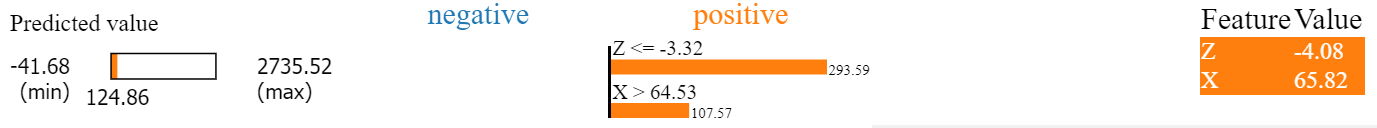
\includegraphics[width=\linewidth]{pics/limexz.png}}
\end{figure}

Стоит отметить, что данная иллюстрация показывает, как сформировалось предсказание под влиянием признаков, если исходно отталкиваться от некоторого среднего значения (среднего предсказания).

LIME отмечает, что оба признака внесли положительный вклад в результат работы модели: значение предсказания выросло примерно на 400 единиц. При этом важно, что признак $Z$ принял значение меньше $-3.32$, а признак $X$ -- значение больше $64.53$. Данные пороги как раз объясняются дискретизацией признаков в алгоритме LIME.

Вернемся к исходному виду зависимости, чтобы сравнить полученный результат с истинной зависимостью. В самом деле, при каждом $X > 64.53$ график функции $y(z)$ выглядит как парабола с ветвями вверх с вершиной в $Z=0$, причем чем больше $X$, тем быстрее возрастают ветви параболы. Соответственно, при любых значениях $Z$, отличных от нуля функция возрастает. Значит, LIME представил правдивый результат: оба признака действительно вносят положительный вклад в значение зависимой переменной, что верно выявила наша модель.